\clearpage
\section{Optical Sensing}
\label{Optical_emitter_receiver}
\subsection{Introduction}
\label{op_intro}
Laser profiling (or \textit{laser altimetry}) is the simplest application of the \acs{LiDAR} technique. The main principle is pretty straightforward; electromagnetic radiation (visible or near-infrared radiation) is emitted towards the Earth's surface by a \acs{laser} and the reflected radiation is detected some time later. By measuring the time delay and knowing the speed of propagation, the range (distance) from the instrument to the surface can be determined. Detailed topographic maps of very high accuracy are produced by airborne or satellite laser altimeter terrain mapping. The unique capabilities of this technique yield more comprehensive and precise topographic information than traditional methods. Airborne laser altimeter data can be used to accurately measure the topography of the ground, even where overlying vegetation is quite dense. The data can also be used to determine the height and density of the overlying vegetation, and to characterize the location, shape, and height of buildings and other man-made structures.


The capacity of any instrument to be able to detect and emit electromagnetic radiation for \acs{laser} altimetry mission depends on optical characteristics, like (wavelength dependent) atmospheric absorption, surface reflectance (ground and oceans) and scattering. These optical phenomenon should be taken into account when multi-angular \acs{laser} altimetry results are wanted. Considering these characteristics, the right instruments can be chosen.

\subsection{Atmospheric and Oceanic Effect}
\label{introAandO}
\subsubsection{Atmospheric Transmission}
\label{introAtmospheric}
For optical signal propagation in the atmosphere, the physical processes dictating the choice of wavelength are summarized in figure \ref{fig:intro_atmosphere} on page \pageref{fig:intro_atmosphere}, which illustrate show the effects of the strong absorption by atmospheric gases act to limit transmission to distinct wavelength regions, or spectral bands.

\begin{figure}[ht!]
\centering
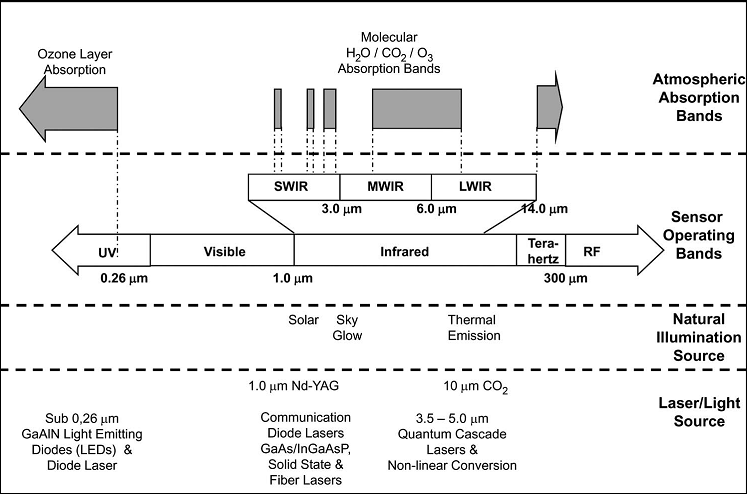
\includegraphics[scale = 0.8]{chapters/img/intro_atmosphere.png}
\caption{A schematic summary illustrating how absorption by various constituents in the atmosphere influences the propagation of light and divides the spectrum into distinct bands.}
\label{fig:intro_atmosphere}
\end{figure}

With in these bands, the atmosphere is relatively transparent and imaging sensor systems can operate efficiently. For wavelengths longer than about one micro-meter, the dominant absorption is related to excitation of molecular vibrations in water vapor and carbon dioxide. When examined in detail, these processes three distinct transmission windows: the near or shortwave infrared bands (\acs{NIR} $\lambda$ ~ 0.7 to 1.1 $\mu$m and \acs{SWIR} 1.1 to 2.5 $\mu$m), the midwave IR band (\acs{MWIR} $\lambda$ ~ 3.3 to 5.0 $\mu$m), and the long-wave IR band (\acs{LWIR} $\lambda$ ~ 8 to 14 $\mu$m). Figure \ref{fig:intro_atmosphere_bands} on page \pageref{fig:intro_atmosphere_bands} shows the absorption and scattering of direct light in the earth's atmosphere.

\begin{figure}[ht!]
\centering
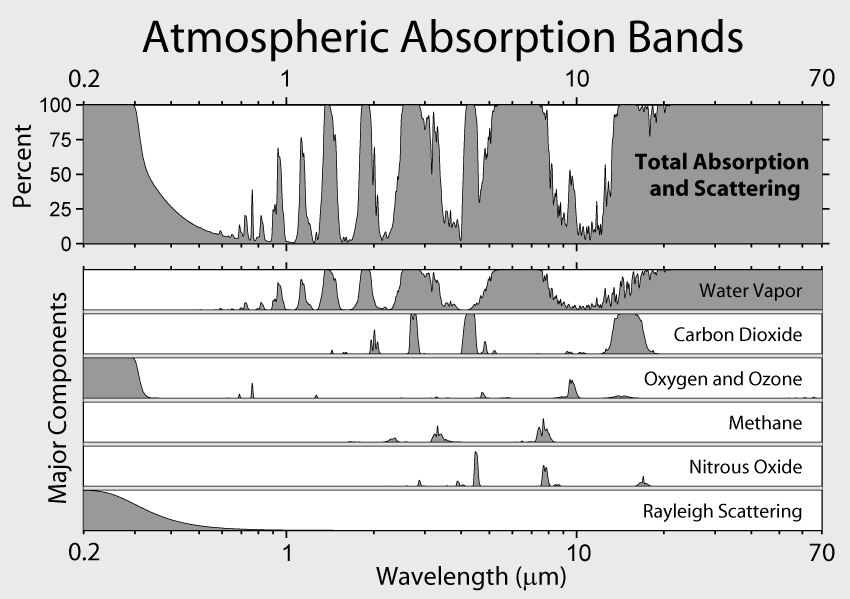
\includegraphics[scale = 0.45]{chapters/img/intro_atmosphere_bands.png}
\caption{Atmospheric Absorption Bands}
\label{fig:intro_atmosphere_bands}
\end{figure}

At the other extreme, for wavelengths much shorter than visible, the same processes responsible for generating airglow limit transmission through the atmosphere. In fact, for wavelengths shorter than ~0.26 $\mu$m [\ac{UV}], these processes are so strong that no solar radiation reaches the ground and the earth's surface is in perpetual darkness (solar-blind). However, this \acs{UV} light does propagate for short distances, all owing sensors designed to respond exclusively in this spectral region to detect many man-made emissions. For example, even when pointed directly at the sun, under conditions where a visible or \ac{IR} system would be completely overwhelmed by the sun's emission, these sensors can detect a UV flash emitted by flames, firearms, or missile plumes. Solar-blind sensors are also of interest because they operate in a region of the spectrum important for detecting certain characteristic florescence associated with biological agents (e.g.,an-thrax) when illuminated by sources operating at even shorter wavelengths. 

\subsubsection{Ocean scattering}
\label{introOcean}
To be able to make any oceanographic elevation model, the incident photons should be scattered by the oceans. This is a particularly important factor for the entire mission, since the coverage of oceans (water in general) is particularly abundant on Earth. The downside of water is the presence of large fractions of absorption in the visible wavelength. This is shown in figure \ref{fig:intro_ocean_penetrate} on page \pageref{fig:intro_ocean_penetrate}. In this picture it can be seen that relatively low wavelengths (or high frequencies) in the visible spectrum (referred to as 'blue') has the highest penetration depth. However, wavelengths in the order of 350 - 450 [nm] have the highest fraction of reflectance on the ocean surface \cite{ocean_scattering}. In comparison, the absorption depth of higher wavelengths, like 'red' (>600 [nm]), has a low value, but almost all radiation with this frequency is absorbed. 

\begin{figure}[ht!]
\centering
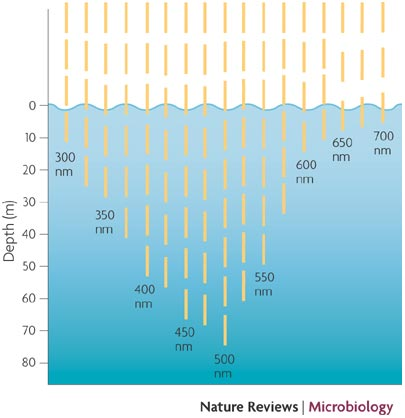
\includegraphics[scale = 0.7]{chapters/img/Ocean_absorption.jpg}
\caption{Light penetration ocean depth with different wavelength}
\label{fig:intro_ocean_penetrate}
\end{figure}

\subsection{Optical Receiver Device}
\label{TOORD}
The main objective of the \ac{ORD} is to detect the individual energy quanta. A large fraction of the photons emitted by the \acs{laser} are not that easy for detection since they are redirected by the atmosphere, spread due to surface scattering or they are simply absorbed partly by either of them. The decrease in photon quantity is really severe considering these factors and that is why a photon detector with comparable high quantum efficiency is required. Since the number of photons actually reaching the perimeter of the \ac{ORD} is usually only in the order of one to ten, the \acs{ORD} has to be able to detect and analyze individual small energy packets, preferably single photons. In this section, general introduction about photon detection is drawn first, then the \acs{laser} wavelength estimation is performed to narrow down wavelength range.After that design option tree is pruned according to the wavelength requirement and technology availability, and there are new approaches after deeply research. Finally the trade off is performed which is split up into trade method, trade criteria and weight factor, followed by trade off summary. The design selection for the optical receiver device is done at the end of the section.

\subsubsection{General Introduction to Photon Detection}
\label{introReceiver}
Photon detection typically occurs in a two-step process: the absorbed photon creates a measurable change in the detector's electrical properties, and the changes is registered in an external read-out integrated circuit (\acs{ROIC}). In general, the detector material responds either \textit{directly} to the incident photon by generating a free charge, with this charge then being responsible for producing the change in electrical properties, or \textit{indirectly}, with the absorbed optical power generating a temperature rise in the detector material, which is responsible for producing the change in electrical properties. In either case, this photon-induced analog signal is registered and amplified in the \acs{ROIC} digitization for further signal processing. 

Additional factors include the detector material \textit{sensitivity} and the detector \textit{device speed of response}. Sensitivity is a measure of how few photons are required to raise the detector output above any background noise level present in the absence of incident light. Response speed is a measure of how faithfully the detector's electrical output responds to changes in the intensity of the input light signal.
\begin{itemize}
	\item Solid-State Photon Detection
Solid-state imaging is based on the physical principle of converting light (photons) into a measurable quantity (electrical voltage, electrical current). Photons falling onto and penetrating into a semiconductor substrate can transfer part of their energy to the substrate by generating electron-hole pairs. For an n-type semiconductor, if the energy content of the photons is high enough, electrons can be released from the valence band and swept into the conduction band, leaving behind a hole in the valence band. To generate an electron-hole pair, the energy of the photons has to be larger than the bandgap of the semiconductor substrate.\cite{photogrammetry}

For reasons of cost and miniaturization, a solid state solution for single photon detection is highly desirable. Figure \ref{fig:intro_receiver1} on page \pageref{fig:intro_receiver1} shows a classification that covers the current state-of-the-art on optical solid-state 3D image sensors. 

\begin{figure}[ht!]
\centering
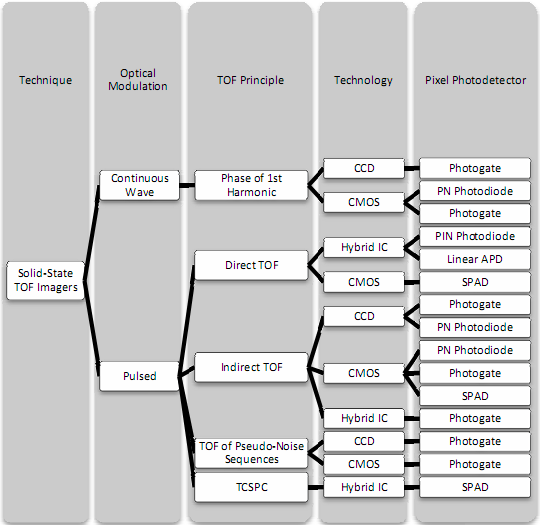
\includegraphics[scale = 1]{chapters/img/intro_receiver1.png}
\caption{Classification of state-of-the-art optical \ac{TOF} image sensors.}
\label{fig:intro_receiver1}
\end{figure}

\item \acs{SPAD}
\ac{SPAD} are solid-state semiconductor devices based on a p-n junction reversed biased at a voltage $V_{a}$ higher than $V_{B}$.

\begin{figure}[ht!]
\centering
\includegraphics[scale = 0.7]{chapters/img/SPAD_Cross-section.png}
\caption{\acs{SPAD} cross-section diagram.}
\label{fig:SPAD_cross-section}
\end{figure}

At this bias, the electric field is so high (higher than 3105 V/cm) that a single charge carrier injected in the depletion layer can trigger a self-sustaining avalanche. The current rises swiftly (sub nanosecond rise-time) to a macroscopic steady level, in the milliampere range. If the primary carrier is photo-generated, the leading edge of the avalanche pulse marks (with picoseconds time jitter) the arrival time of the detected photon. The current continues until the avalanche is quenched by lowering the bias voltage VD down to or below $V_{B}$: the lower electric field is not able any more to accelerate the carriers to impact-ionize with lattice atoms, therefore current ceases. In order to be able to detect another photon, the bias voltage must be raised again above breakdown.\cite{SPAD_intro}

\end{itemize}


\subsubsection{Wavelength estimation}
\label{introReceiver}
Laser wavelength is one of the most important parameters influencing the whole design of photon detection device and \acs{laser} emitter choosing. Different emitter wavelengths have different photon detection efficiency or probability to photon receiver. To choose which type of \acs{laser} is feasible, it is best to start with which wavelength the receiver can detect.

According to the photon detection probability distribution diagram for \acs{SPAD} and \acs{MPD} in figure \ref{fig:SPAD_efficiency} and \ref{fig:MPD_efficiency} on page \pageref{fig:SPAD_efficiency} and \pageref{fig:MPD_efficiency}, the general most sufficient wavelength range is between 400nm to 900nm. 

\begin{figure}[ht!]
\centering
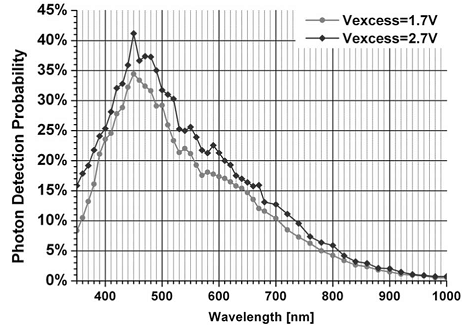
\includegraphics[scale=1]{chapters/img/SPAD_efficiency.png}
\caption{\acs{SPAD} photon detection probability as a function of wavelength for two values of excess bias voltage}
\label{fig:SPAD_efficiency}
\end{figure}

\begin{figure}[ht!]
\centering
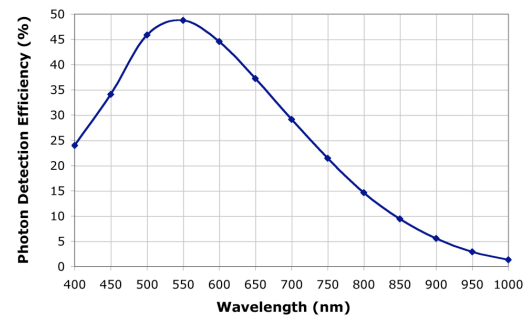
\includegraphics[scale=1]{chapters/img/MPD_efficiency.png}
\caption{\acs{MPD} photon detection probability as a function of wavelength}
\label{fig:MPD_efficiency}
\end{figure}

There are not much qualified \acs{laser}s can be considered below the wavelength 400nm, and the photon detection probability is insufficient if the wavelength goes above 900nm. In order to narrow the wavelength range, the atmospheric transmittance versus photon detection efficiency ratio is introduced, which means that larger ratio indicates larger chance the receiver can detect photon. The actual formula to calculate the ratio is R = transmittance$^{2} \times$ photon efficiency. The transmittance is squared because the light go through the atmosphere twice. Calculate all ratio between wavelength 400nm to 900nm by interval 25nm, and plot the ratios in figure \ref{fig:wavelength_estimation} on page \pageref{fig:wavelength_estimation}. From the graph, it is easy to narrow down the wavelength range to 425nm-500nm.  The following sections will give brief trade-offs between \acs{laser} emitters and receivers.

\begin{figure}[ht!]
\centering
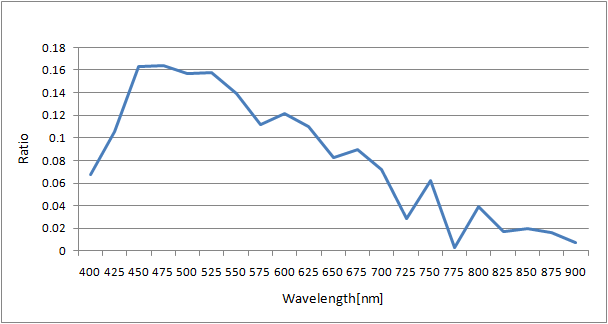
\includegraphics[scale=1]{chapters/img/wavelength_estimation.png}
\caption{Ratio of atmospheric transmittance versus photon detection efficiency}
\label{fig:wavelength_estimation}
\end{figure}

\subsubsection{Receiver Prune}
\label{TOReceiverP}
In the design option tree, the GLAS branch is obviously dropped out, since we are trying to improve the whole concept. Meanwhile, the \ac{MPD}'s single-photon detection modules branch has different quantum efficiency for different wavelength, which means MPD could be a good option for the blue laser detector with 35\% efficiency. The \ac{SPAD} chip could be a new approach since it has reasonable high quantum detect efficiency at laser wavelength 425nm to 500nm. Both \acs{MPD} and \acs{SPAD} are not optimal for \acs{NIR} or \acs{IR} laser detect with low quantum efficiency around 1\%, So it means the mission mainly focus on single wavelength.

The pruned design option tree for the laser detector can be seen in figure \ref{fig:PrunedReceiver} on page \pageref{fig:PrunedReceiver}.

\begin{figure}[ht!]
\centering
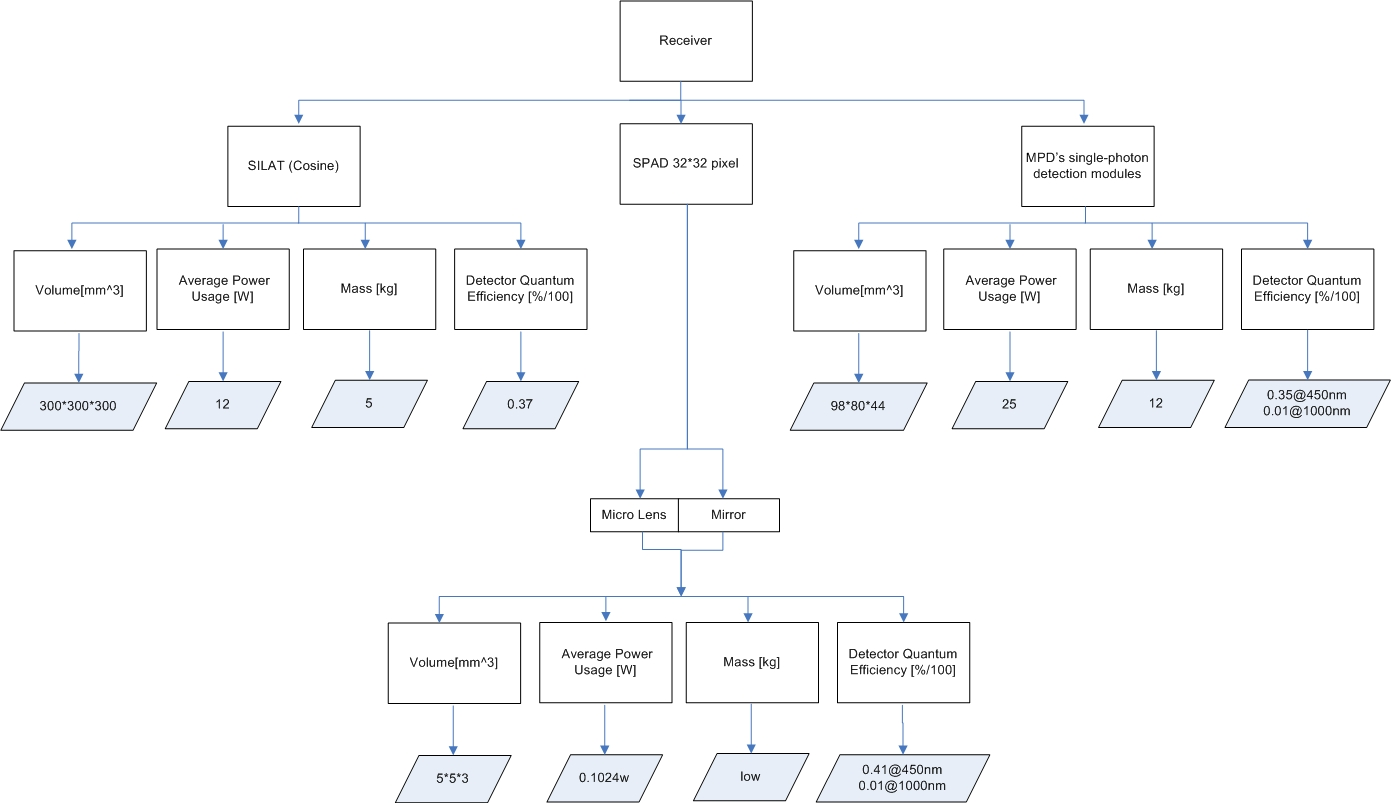
\includegraphics[scale=0.7, angle=90]{chapters/img/DOTreceiverPruned.jpg}
\caption{The pruned design option tree for the Laser receivers}
\label{fig:PrunedReceiver}
\end{figure}

\subsubsection{Trade Method}
\label{TOReceiverM}
There are mainly four options after pruning and each has different strong points and weak points due to different configuration and structure. 

The first option is \ac{SILAT}, which combines two optical cameras with a low-power photon-counting laser altimeter. It means that \acs{SILAT} operates both pulse laser and photon detector, and it need to be configured as only a photon detector(more information are needed about the configuration). The main strong point is that \acs{SILAT} should has relative higher reliability since it is designed suitable for space mission like spectral imagery and satellite topographic study. 

\ac{MPD}'s photon detection efficiency is obtained through the use of epitaxial silicon \ac{SPAD} and patented \ac{IAQC}, which is specifically designed and optimized for photon counting. The main drawback is that it is difficult to achieve the precise ground resolution due to diffraction, and it also has large volume and power consumption.

The final option is use a 32$\times$32 pixel array with in-pixel photon counting, which also use \acs{SPAD} but in \ac{CMOS} technology \cite{SPAD}. It has the highest quantum efficiency for blue laser(425nm to 500nm), but only 2\% of the chip area can detect the quanta. In this case, micro lenses or faceted mirrors are used in order to collect most of the incoming quanta focus on such a small area. The solution draft design is shown in figure \ref{fig:diagram_Rgeneral} on page \pageref{fig:diagram_Rgeneral}. Both designs use the parabolic mirror placed at certain position to the small \acs{SPAD} chip with a specified curvature, then the prism barrier is designed to filter other noise lights except wavelength about 425nm to 500nm blue light. After that, different receiver assemblys are designed.

\begin{figure}[ht!]
\centering
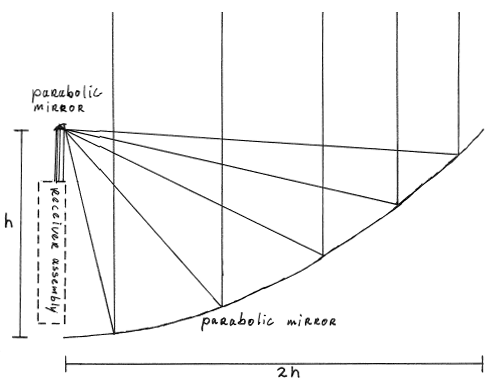
\includegraphics[scale = 0.6]{chapters/img/DiagramReceiverGeneral.png}
\caption{The diagram of the parabolic mirror}
\label{fig:diagram_Rgeneral}
\end{figure}

The draft design diagram of assembly micro lenses is shown on figure \ref{fig:diagram_Rmicrolenses} on page \pageref{fig:diagram_Rmicrolenses}. The micro lenses are placed just above the \acs{SPAD} chip to focus light source on the specific pixel 2\% area. These lenses can increase the sensing area by factor of 5, which means 10\% area can be used for detection. On the other hand, the micro lenses could be very heavy due to the high density of the lens material, and it could also has the risk of falling off due to vibration during lunching and boosting. Since the micro lenses is manufacturing in scale of micro meters, it could be an extra problem to achieve the precision.

\begin{figure}[ht!]
\centering
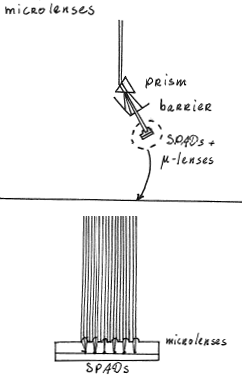
\includegraphics[scale = 0.6]{chapters/img/DiagramReceiverAssemblyMicrolenses.png}
\caption{The diagram receiver assembly micro lenses}
\label{fig:diagram_Rmicrolenses}
\end{figure}

Another way to increase the receiving efficiency is using the faceted mirror such as the figure \ref{fig:diagram_Rfaceted mirror} on page \pageref{fig:diagram_Rfaceted mirror} shown. Instead of the heavy micro lenses, the multi-faceted elliptical mirror can be placed to achieve the focusing. In this way, the sensing area can be increase enormously from 2\% to around 80\%. Meanwhile, faceted mirror is manufacturing in scale of mini meters, so fabrication precision can be achieved.

\begin{figure}[ht!]
\centering
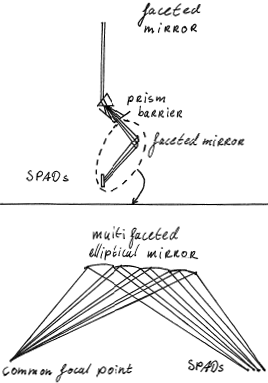
\includegraphics[scale = 0.6]{chapters/img/DiagramReceiverAssemblyFacetedMirror.png}
\caption{The diagram receiver assembly faceted mirror}
\label{fig:diagram_Rfaceted mirror}
\end{figure}

\subsubsection{Trade Criteria}
\label{TOReceiverC}
In the last paragraph, the general trade off method is elaborated but not in quantity way. It is more precise and clear to give some trade criteria to compare between options, which can be graded from 1-10 (worse to best) to indicate each criterion performance. Mass, power, volume are criteria considered as design of a constellation of micro or nano satellites. The criteria such as efficiency, reliability, resolution and \ac{FOV} are defined whether the receiver can detect photon or not and how precision it could be. Last but not the least, Cost, lifetime and availability need to be noticed generally in each subsystem.

\subsubsection{Weight Factor}
\label{TOReceiverWF}
Weight factor is given differently to each criterion due to mission objective and instrument performance requirement. Lifetime is the top objective and the efficiency determines the photons can be detected or not, so both are given as maximum of 10. Power, mass, volume are important since micro or nano receivers are considered. Meanwhile resolution, reliability and \acs{FOV} are also important to ensure the system can perform continuous accurate measurements. The mission objective is mainly about feasibility study, so cost and availability should not be the essential part.

\subsubsection{Trade summary}
\label{TOReceiverS}
The trade off table is shown in figure \ref{fig:receiver_tradeoff} on page \pageref{fig:receiver_tradeoff}. The \acs{SPAD} plus micro lenses and faceted mirror designs have the much higher grades than \acs{SILAT} or \acs{MPD}. The \acs{SPAD} with micro lenses has lowest grade for efficiency, which is mentioned in early chapters, because the lenses which is manufactured in scale of micro meters can only increase the efficiency by factor of 5. On the other hand, the faceted mirror can increase the fill field from 2\% to 80\%, that is why faceted mirror has much larger efficiency. The \acs{SPAD} with faceted mirror design has the large advantages on power comsuption(100$\mu$W), mass(tens of grams) and volume($5\times5\times3[mm^{3}]$) comparing to either \acs{SILAT} or \acs{MPD}, that is much more realistic and practical if the swarm of receiver satellites are in scale of micro or even nano. The \acs{SPAD} with faceted mirror turns to be the best option after all, and it should be further invested later on in detail design.

\begin{figure}[ht!]
\centering
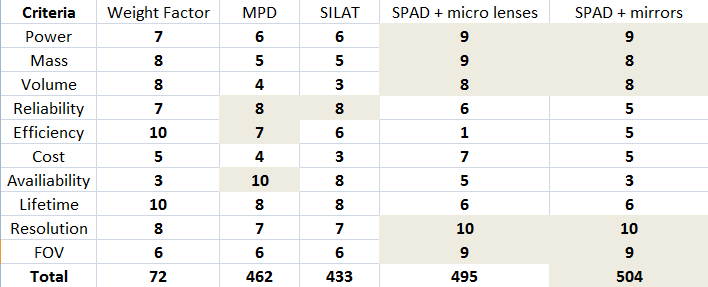
\includegraphics[scale = 1]{chapters/img/Receiver_tradeoff.png}
\caption{The receiver trade off table}
\label{fig:receiver_tradeoff}
\end{figure}

\subsection{Optical Emitting Payload}
	\label{mtDOLSR}
\acs{LiDAR} altimetry missions are dependent on electromagnetic or acoustic radiation transmission. In order to make a multi-angular \acs{DEM}, a \ac{laser} system is chosen. Since there are myriad types of \acs{laser}s, it is crucial to understand the basics behind this technology.  

	\subsubsection{Optical Transition}
\cite{laser_fundamental}Solving the time-dependent Schrodinger equation for free electrons (represented as harmonic oscillators) shows the presence of certain energy gaps, i.e. the existence of quantisized energy states, according to quantum mechanics. In a more mathematical view, the quantum particles in a particular system share the same eigenfunction, but have different eigenvalues. Among energy states, the states with the lowest energy is the most stable one. If they are \textit{excited} by thermal energy, light or electron beams, the electrons absorb these energies and transit to a higher energy state. These transitions of the electrons from low energy states to high energy states are called \textit{excitations}. Higher energy states, however, are unstable. As a result, the electrons in higher energy states transit to lower energy states in certain \textit{lifetimes}. These transitions of the excited electrons from high energy states to low energy states are referred to as \textit{relaxations}. In the recombination of negatively charged electron and positively charged holes (exciton pairs) there are radiative (emission of photons) and non-radiative (phonon emission through crystal lattice) recombinations.

	\subsubsection{Exciton Dynamics}   
Figure \ref{fig:laser} on page \pageref{fig:laser} schematically shows the possible radiations and absorption. In the radiations, there are spontaneous emission and stimulated emission. Spontaneous emission is a radiative process in which an excited electron decays in a certain lifetime and a photon is emitted. In contrast, with stimulated emission, an incident photon induces a radiative transition of an excited electron. The emitted photon due to stimulated emission has the same wavelength, phase, \textbf{k}-vector, polarization and direction. Therefore, the light generated is highly monochromatic, coherent and directional. As a result of the two photons generated from this process, the electromagnetic radiation is amplified. These quantum particles can on their turn start the same procedure on different electrons. 

\begin{figure}[ht!]
\centering
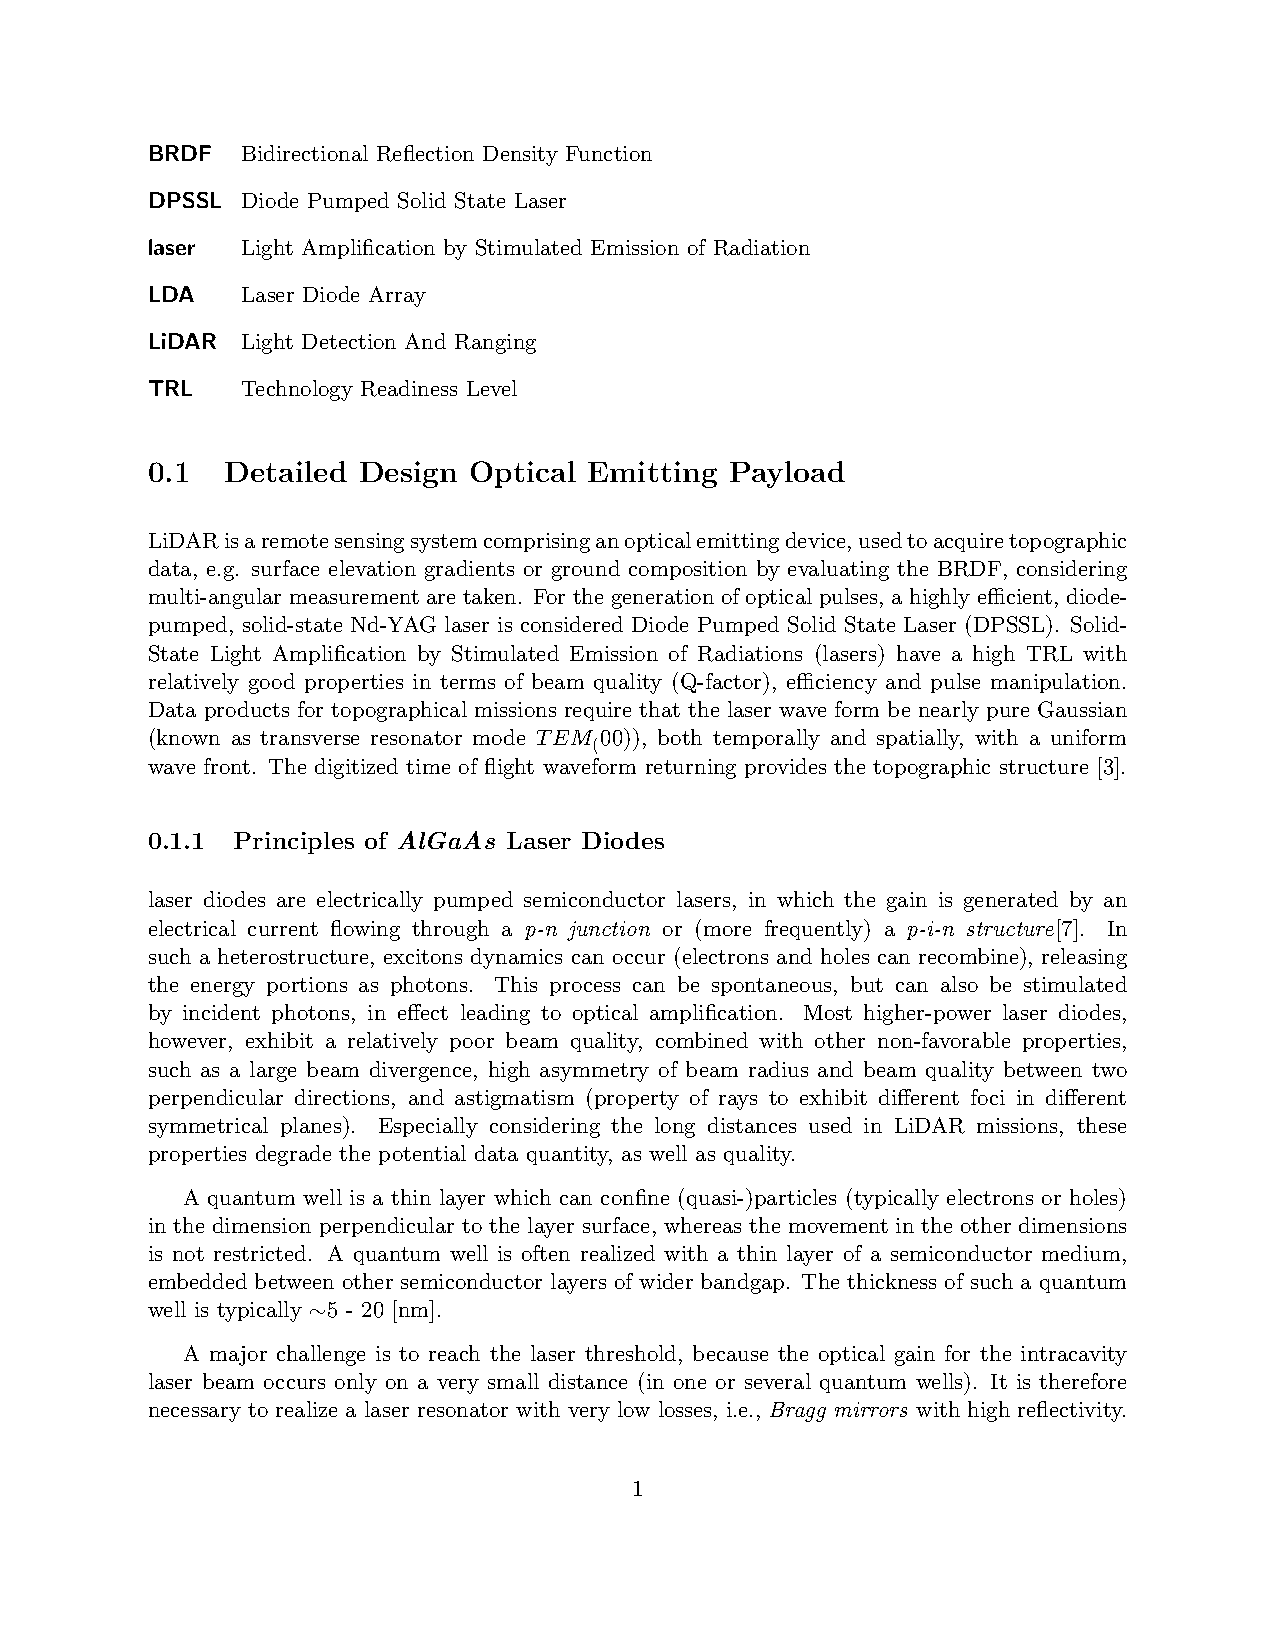
\includegraphics[scale=0.4]{chapters/img/laser.png}
\caption{Left: individual energy quantum energy levels occupied with individual wave equation. Optical transitions given in random electron orbit; emission and absorption could take place at any energy level. Right: Einstein coefficients for optical transmission. 'J' represents the photon density in \textbf{k}-space. Spontaneous emission is independent on photon density.}
\label{fig:laser}
\end{figure}
 
When a light is incident on a material, the stimulated emission and the absorption simultaneously take place. In thermal equilibrium, there are more electrons in a lower energy state than in a higher one, because the lower energy state is more stable. In order to obtain a net optical gain, the number of electrons in a higher energy state should exceed the number of electrons in a (relative) lower energy level. This condition is referred to as \textit{population inversion}, because the electron population is inverted compared with that in thermal equilibrium. 
 
 	
	\subsubsection{Laser Geometry}
The \acs{laser} oscillator uses fractions of the spontaneous emission as the optical input and amplifies the fractions by the stimulated emission under population inversion. Once the optical gain exceeds the optical losses, laser oscillations take place. An oscillator has a gain and amplifies an input. To feed back light, \textit{optical resonators} or \textit{optical cavities}, which are composed of reflectors or mirrors, are adopted. Due to this configuration (which is used by pretty much all \acs{laser} types), characteristics of \acs{laser}s are affected by the optical gains and optical resonators. 

\begin{figure}[ht!]
\centering
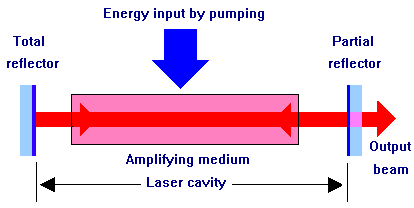
\includegraphics[scale=0.6]{chapters/img/laser cavity.png}
\caption{General layout of a \acs{laser}. \acs{laser} cavity with fully reflecting mirror (left) and partially reflected mirror (right). Under the stimulation of population inversion lasing action occurs due to optical reflection.}
\label{fig:laser_cavity}
\end{figure}

	\subsubsection{Efficiency}
Unfortunately, the induced power (pump power) cannot be perfectly transmitted to the electromagnetic radiation, i.e. the efficiency of the \acs{laser} cavity and \acs{laser} resonator are not equal to 100 percent. A number of mechanisms cause this decrease in efficiency:
	\begin{enumerate}
		\item{Cavity Losses}
		\item{Optic Misalignment}
		\item{Optical Transition}
	\end{enumerate} 

	\subsubsection{Pulsed vs Continuous Waves}
Without any alterations of the electromagnetic radiation created by the stimulated emission within the \acs{laser} cavity, the radiation, once in equilibrium, behaves like a continuous wave. The energy within this wave is equal to the pumper power minus the \textit{round-trip inter cavity power losses}. However, the wave can also be pulsed. The pulse energy Ep is simply the total optical energy content of a pulse. For regular pulse trains, the pulse energy is often calculated by dividing the average power (measured e.g. with a powermeter) by the pulse repetition rate [Hz]. However, this is a valid procedure only if the energy emitted between the pulses is negligible. There are cases where, e.g., a mode-locked laser emits a pulse train together with a low-level background emission. Even if the background power level is far below the peak power, the background can significantly contribute to the average power. 

The pulse energy together with the pulse duration is often used to estimate the peak power of pulses. Conversely, temporal integration of the optical power results in the pulse energy.

Typical pulse energies from Q-switched lasers range from microjoules to millijoules, and for large systems to multiple joules or even kilojoules. Mode-locked lasers achieve much lower pulse energies (picojoules, nanojoules or sometimes several microjoules) due to their high pulse repetition rates and sometimes due to limiting nonlinear effects in the laser resonator. Much higher energies of ultrashort pulses can be achieved by amplifying pulses at a lower repetition rate.

The pulsed configuration can be beneficial in \acs{laser} altimetry missions, since individual pulses can be detected and analyzed. Hence, the footprint can be subdivided and the analyses of the incoming photons (energy packages) can result into a more detailed \acs{DEM}.  

	\subsubsection{Blue Laser Types}
In the baseline report, a number of \acs{laser}s was listed. Considering the fact that the receiver should be able to detect single photons, the actual \acs{OED} characteristics are dependent on the receiver. Since the receiver efficiency is a function of wavelength, the appropriate wavelength should be transmitted. Since \acs{laser}s show discrete wavelength characteristics, the type of \acs{laser} should be determined from this criteria.

The analysis of the chosen wavelength is determined in chapter wavelength estimation.

The receiver characteristics show that the laser should have a wavelength in the interval of 425 - 500 nm (within visible spectrum designated as 'blue'). Hence, every \acs{laser} with different wavelengths is not viable for this analysis.

Potential \acs{laser} types for this altimetry mission:

\textit{Helium-Cadmium (He-Cd) \acs{laser}}\\
Wavelength: 441.6 [nm]\\
Gain medium type: Gas

\textit{Neodymium-doped Yttrium Aluminium (Nd-YAG) \acs{laser}}\\
Wavelength: 946 [nm] (473 [nm] with frequency doubling)\\
Gain medium type: Solid-State

\textit{Argon (Ar) \acs{laser}}\\	
Wavelength: 454.6 [nm]\\
Gain medium type: Gas

\textit{\acs{laser} diode sytems}\\
Wavelength interval 400 - 480 [nm] (tunable). The wavelength interval of this kind of \acs{laser} is excellent, but they are difficult to produce for high output power and long (> year) lifetimes. Since the determined lifetime in this mission exceeds this \acs{laser} lifetime, this \acs{laser} is not part of the trade-off.
	
	\subsubsection{Trade-off}
\begin{figure}[ht!]
\centering
\includegraphics[scale=1]{chapters/img/laser_tradeoff.png}
\caption{\acs{laser} trade off table}
\label{table:laser_tradeoff}
\end{figure}

Table \ref{table:laser_tradeoff} on page \pageref{table:laser_tradeoff} shows the trade-off for the different \acs{laser}s. The most important  criteria and the ones that clearly need some explanation, are discussed in more detail in this section for the different gain media. 
	
\textbf{Wavelength ratio}. The emitted wavelength is an important factor for the possibility of photon detection as function of atmospheric absorption and receiver efficiency. Considering the wavelength dependency of these last two terms, the laser types have a different wavelength ratio (see: chapter receiver).

\textbf{Cost}. Gas \acs{laser}s in general are relatively cheap , because of the high \acs{TRL} and the relatively simple optical subsystems within the \acs{laser} cavity. The costs of the optical emitting payload is considered to have a low weight factor. The typical cost estimation for a gas \acs{laser} equals \$20,000 and \$30,000, whereas the solid-state \acs{laser} can cost almost double (\$45,000 - \$50,000). However, since the total cost of the mission are in the order of 200 M\$, this difference is negligible.
 
\textbf{Minimum Pump Power}. \cite{lasertech}The threshold pump power of a laser is the value of the pump power at which the laser threshold is just reached, usually assuming steady-state conditions. At this point, the small-signal gain equals the losses of the laser resonator. For an optically pumped laser, the definition of threshold pump power may be based either on the incident or absorbed pump power. A low threshold power requires low resonator losses and a high gain efficiency.

Calculation for the \acs{laser} types:

\begin{center}
$p_{p.th} = \frac{I_{rt}}{\eta_{p}\tau_{2}\sigma_{em}}$
\end{center}

P: Threshold power [W], I: Round-trip intercavity power loss [W], $\eta$: Pump efficiency, $\tau$: Upper laser level lifetime, $\sigma$: Stimulated emission cross section

\textit{Helium-Cadmium}
Pumping efficiency: 0.82\\
Upper \acs{laser} level lifetime [s]: $7.1\cdot10^{-7}$\\
Round trip power losses [$10^{-28} W$]: 2.357 \\
Stimulated emission cross section [$m^{2}$]: $9.0\cdot10^{-18}$\\
Minimum Pump Power [mW]: 45 

\textit{Nd-YAG}
Pumping efficiency: 0.92\\
Upper \acs{laser} level lifetime [s]: $2.30\cdot10^{-6}$\\
Round trip power losses [$10^{-28} W$]: 5.01\\
Stimulated emission cross section [$m^{2}$]: $2.8\cdot10^{-23}$\\
Minimum Pump Power [mW]: 75

\textit{Argon}
Pumping efficiency: 0.82\\
Upper \acs{laser} level lifetime: $1.0\cdot10^{-8}$\\
Round trip power losses:  2.787\\
Stimulated emission cross section [$m^{2}$]: $2.6\cdot10^{-16}$\\
Minimum Pump Power [mW]: 50

\textbf{Repetition Rate Manupilation}. To be able to create short pulses, the electromagnetic radiation present due to stimulated emission should be altered. This can be done with multiple mechanisms, like Q-switching, mode-locking or mechanical interference. However, only two of these (Q-switching and mechanical interference) can be used with gas \acs{laser}s, giving rise to only moderately short pulses. Mode-locking, which is possible for solid-state \acs{laser}s, allows the user to creates shorter pulses and next to that, if active mode-locking is considered, the pulses can actually have a temporal deviation. 
 
\textbf{Volume and mass}. 
The mass and volume are particularly dependent on the \acs{laser} cavity length, which equals 0.1 - 0.15 [m] for the solid state-laser and 0.25 - 1.5 [m] for a particular gas \acs{laser}. However, the solid-state \acs{laser} usually exhibits more optical components, increasing the weight.  

\textbf{Chemical Stability}. The use of gas as gain medium can alter and decrease the optical properties of the mirrors. The quality of the internal \acs{laser} components can be decreased and hence, the lifetime is lower.   

\textbf{Thermal Control}. Operational temperatures for the gas \acs{laser} are in the order of 573 [K] (Argon and He-Cd temperature interval as well), whereas the operational temperature for the solid-state \acs{laser} is 300 [K] with a relatively larger operational temperature interval compared to the gas \acs{laser} configuration.  

\textbf{Efficiency}. The Argon \acs{laser} has very poor power efficiency, hence the transfer from the pump energy to the actual electromagnetic radiation is low, giving rise to (very low efficiency). The efficiencies (as described as above) are pretty equal for the other two options, around 40%.
 
	
	\subsubsection{Thermal Control Solid-State \acs{laser}}
\subsection{Laser Thermal Control}
	\label{mtLSRthermal}
The functioning of the optical payload is dependent on a specific temperature interval, so in order to be able to meet the top level requirements, thermal control considerations for the emitter and receiver should be taken into account. 

\subsubsection{Thermal Physics}
	\label{mtLSRthermalphysics}
Two important mechanisms of thermal conductivity are (free) electron translation (crystal momentum) and phonon states. A phonon (state) is a quantum of acoustic energy, analogous to the quantum of electromagnetic radiation, the photon. Thermal excitations in a crystal or in an elastic medium can be described as a population of phonons. Basically, phonons represent a mode of vibration occurring in a rigid crystal lattice. Since, on one side, individual electrons in a crystal lattice are bound in terms of quantisized energy levels and on the other side they are interconnected to neighboring particles by electric force (attraction or repulsion) as a function of distance, in most solids the energy given to lattice vibrations is the dominant contribution to the heat capacity, i.e. induced thermal energy is converted to a change in rate of crystal momentum or phonon state, which can be represented by a difference in internal energy. In this light, the terms 'thermal energy' and 'internal energy' represent the same quantity. 

From an electron point of view, a change in temperature (or any change in state variable) represents the quest for a new thermal equilibrium situation. Since electrons are fermions, their orbit population is described by the temperature dependent Fermi-Dirac distribution. Fermions show the tendency to occupy the lowest energy levels and since they are limited due to Pauli's exclusion principle, which states no identical fermion with equal intrinsic spin can occupy the same energetic orbit, not every electron can be in the ground state. Increasing the internal energy will therefor represent thermal excitation.  

\subsubsection{Theoretical Thermal Limits For Lasers}
	
\begin{itemize}
	\item Gain Medium Thermal Overloading
Thermal overloading can be divided to the temperature interval at which electron excitation is impossible and the interval at which permanent crystal lattice deformation occurs.

\textit{Short term temperature increase (T $<$ 323.15K)}
To begin with the first phenomenon, in order to excite any electron, the conduction band should not be completely filled in thermal equilibrium. Any excitation, so also stimulated excitation, would be impossible and hence no lasing action would occur. In the real world, a small part of the electrons will give rise to stimulated emission since not all electrons would occupy the highest energy bands, considering the temperature to increase. However, population inversion would not be present. If the temperature is decreased afterwards, the gain material would be able to provide lasing action, making it an short-term problem with no permanent significance. 

\textit{Long term temperature increase (T $>$ 323.15K)}
However, if the induced (thermal) energy is increased even further, the crystal lattice can eventually alter in time. This crystal lattice deformation not only implies the gain material, but all optical subparts, causing possible lasing failure. Recrystallization of the material can occur if the upper limit of the temperature interval is reached, giving birth to long-term (partial) failure. Another longterm effect is thermal fatigue for parts within the laser.
	
\item Thermal Lensing
\textit{Long term temperature increase (T $>$ 303.15K)}
Particularly in high-power lasers, the appearance of a temperature-gradient in the gain medium often causes a significant 'thermal lens'. The gain medium has higher internal energy on the beam axis, typically causing some transverse gradient of the refractive index according to the temperature-dependent Sellmeier equation. 

\begin{figure}[ht!]
	\begin{center}
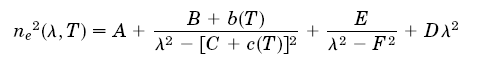
\includegraphics[scale=0.5]{chapters/img/TISE.png}	
\caption{Refractive index as function of radial position, where the Sellmeier coefficients A, B, C, D, E, and F are constants dependent on gain material, c and b are temperature dependent, T is the temperature in degrees centigrade, and l is the wavelength in micrometers.}
\label{thermal_lensing}
\end{center}
\end{figure}

Thermal lensing occurs due to the combined effect of the thermal expansion and thermally induced refractive index change. The magnitude of the thermal lensing scales proportional to the power absorbed by the gain medium and the thermo-optic coefficient of the material, and inversely proportional to the thermal conductivity of the material. 

The Sellmeiser equation could also be used for the change in refractive index for all other optical subparts in the laser, like the lenses. Since the refractive index will change due to the change in temperature, this has to be taken into account.   

\begin{figure}[ht!]
	\begin{center}
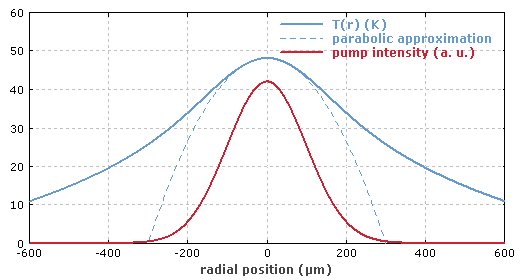
\includegraphics[scale=0.7]{chapters/img/thermal_lensing.png}	
\caption{Transverse pump intensity distribution (red) and thermal profile (blue). The temperature profile is approximately parabolic only near the center of the crystal.}
\label{thermal_lensing}
\end{center}
\end{figure}

External induced thermal energy can therefor cause the formation of a thermal lens, causing the beam quality to alter. Especially beam divergence tends to decrease by the formation of a thermal lens, i.e. the change in refractive index change per unit temperature (dn/dT) should be kept within limits. The absence of thermal control can even lead to non-localized thermal lensing, since temperature-gradients can be localized away from the principal axes. 

\item Multi-Phonon Transitions
\textit{Long term temperature increase (T $>$ 353.15K)}
The upper-state lifetime (the lifetime of the population of the upper laser level) can be strongly reduced by decay processes which involve the simultaneous emission of multiple phonons. Multiple phonons are typically required for such transitions because the energy of a single phonon is not sufficient to match the difference in level energies. The rate of multi-phonon transitions decreases with the increasing number of phonons required. Temperature-gradients can influence the phonon transition and hence influence the the upper-state lifetime, decreasing the beam quality. 

\item Dielectric Transmission
\textit{Long term temperature increase (T $>$ 313.15K)}
Optically absorbing layers (dielectric transmission decrease) can form on the exit face of the fully reflective mirror and on the doubling crystal, resulting in a decay of output power. The absorbed optical energy creates thermal gradients with which affects phase matching and hence lowering the beam quality. 

\item Limit in Electron Movement
\textit{Long term temperature decrease (T $<$ 273.15K)}
If the internal energy decreases to much, the exciton dynamics would alter, i.e. electrons will not be able to be excited to higher energy levels. This temperature dependent tendency is caused by the Boltzmann distribution, giving rise to an increase of potential energy at the lowest energy level. 
\end{itemize}	


\subsubsection{Thermal Control}
	\label{mtLSRthermalcontrol}
As seen in the previous paragraphs, the temperature interval for proper lasing action roughly equals 273.15 $<$ T [K] $<$ 313.15. Since the thermal environmnent is extremely harsh (extremely cold background temperature, intense solar radiation, sudden loss of temperature in shadow and the presence of vacuum), thermal control considerations should be taken into account. 

